\documentclass[10pt,a4paper]{article}
\usepackage[margin=15mm]{geometry}
\usepackage{kotex}
\usepackage{fontspec}
\usepackage{booktabs}
\usepackage{tabularx}
\usepackage{pgfplots}
\usetikzlibrary{calc}
\usepackage{xcolor}
\usepackage{hyperref}
\pgfplotsset{compat=1.18}
\setmainfont{Apple SD Gothic Neo}[BoldFont={* Bold}]
\setmonofont{Menlo}[Scale=0.84]
\definecolor{tborange}{HTML}{FF6F00}
\definecolor{cblue}{HTML}{1F77B4}
\definecolor{corange}{HTML}{FF7F0E}
\definecolor{cgreen}{HTML}{2CA02C}
\definecolor{call}{HTML}{3949AB}

\title{\textbf{TensorBoard 기준 학습·평가 지표 보고서 (ROC/FROC · F1 Score · Scalars)}}
\author{Totalcare KITTI YOLO11m @ 960 (v2\_improved)}
\date{2026-11-14}

\begin{document}
\maketitle
\vspace{-8mm}

\noindent\textbf{대상 디렉터리:} \texttt{results/v2\_improved/outputs/train\_results/} \\
\textbf{원본 실행:} Kaggle 2$\times$ Tesla T4 DDP (\texttt{epochs=40}, Early Stop \texttt{ep=24}, Best \texttt{ep=12}) · Val \texttt{832} imgs / Test \texttt{1,608} imgs

\section*{1. TensorBoard SCALARS / TIME SERIES 요약 및 F1 Score 추이}
\begin{itemize}
  \item \textbf{Val Eval Operating Point (\texttt{best.pt}):} Precision \textbf{0.7170}, Recall \textbf{0.4822}, \textbf{F1 = 0.5766} (v1 Baseline \texttt{0.4971} 대비 \textbf{+0.0795}), mAP@0.5 = \textbf{0.5235}
  \item \textbf{Test Eval Operating Point (Held-out 0013/0016/0019):} Precision \textbf{0.6732}, Recall \textbf{0.4037}, \textbf{F1 = 0.5047}, mAP@0.5 = \textbf{0.4269}
  \item \textbf{Peak F1 on Confidence Sweep:} Val \textbf{0.555} @ conf \texttt{0.191}, Test \textbf{0.487} @ conf \texttt{0.322}
\end{itemize}

\begin{center}
\begin{tikzpicture}
\begin{axis}[
  width=0.92\textwidth, height=5.4cm,
  title={Epoch별 F1 Score · Precision · Recall · mAP@0.5 (v2 YOLO11m @ 960)},
  xlabel={Epoch}, ylabel={Score},
  xmin=1, xmax=24, ymin=0.25, ymax=0.85,
  grid=both, legend pos=south east, legend columns=4,
  tick label style={font=\footnotesize}, label style={font=\small}
]
\addplot[color=tborange, thick, mark=*, mark size=1.3pt] coordinates {(1.0000,0.4091) (2.0000,0.4672) (3.0000,0.4545) (4.0000,0.4178) (5.0000,0.4835) (6.0000,0.5223) (7.0000,0.5032) (8.0000,0.5366) (9.0000,0.5480) (10.0000,0.5375) (11.0000,0.4497) (12.0000,0.5759) (13.0000,0.5572) (14.0000,0.5480) (15.0000,0.4847) (16.0000,0.5087) (17.0000,0.5119) (18.0000,0.5125) (19.0000,0.6008) (20.0000,0.5131) (21.0000,0.5382) (22.0000,0.5190) (23.0000,0.5368) (24.0000,0.5273)}; \addlegendentry{F1(B)}
\addplot[color=cblue, thick, dashed] coordinates {(1.0000,0.4067) (2.0000,0.5150) (3.0000,0.5028) (4.0000,0.4814) (5.0000,0.5063) (6.0000,0.5868) (7.0000,0.5806) (8.0000,0.6357) (9.0000,0.7218) (10.0000,0.6701) (11.0000,0.5375) (12.0000,0.7166) (13.0000,0.6833) (14.0000,0.6593) (15.0000,0.5853) (16.0000,0.6034) (17.0000,0.6709) (18.0000,0.5892) (19.0000,0.7905) (20.0000,0.6305) (21.0000,0.6805) (22.0000,0.6337) (23.0000,0.6654) (24.0000,0.6714)}; \addlegendentry{Precision(B)}
\addplot[color=cgreen, thick, dotted] coordinates {(1.0000,0.4114) (2.0000,0.4276) (3.0000,0.4147) (4.0000,0.3691) (5.0000,0.4627) (6.0000,0.4705) (7.0000,0.4440) (8.0000,0.4642) (9.0000,0.4416) (10.0000,0.4487) (11.0000,0.3865) (12.0000,0.4814) (13.0000,0.4703) (14.0000,0.4689) (15.0000,0.4137) (16.0000,0.4397) (17.0000,0.4139) (18.0000,0.4536) (19.0000,0.4845) (20.0000,0.4325) (21.0000,0.4451) (22.0000,0.4394) (23.0000,0.4498) (24.0000,0.4341)}; \addlegendentry{Recall(B)}
\addplot[color=call, thick] coordinates {(1.0000,0.4074) (2.0000,0.4847) (3.0000,0.4259) (4.0000,0.4001) (5.0000,0.4516) (6.0000,0.4809) (7.0000,0.4686) (8.0000,0.4784) (9.0000,0.4778) (10.0000,0.4886) (11.0000,0.4136) (12.0000,0.5231) (13.0000,0.4944) (14.0000,0.4993) (15.0000,0.4281) (16.0000,0.4525) (17.0000,0.4522) (18.0000,0.4654) (19.0000,0.5297) (20.0000,0.4537) (21.0000,0.4682) (22.0000,0.4560) (23.0000,0.4720) (24.0000,0.4539)}; \addlegendentry{mAP@0.5(B)}
\end{axis}
\end{tikzpicture}
\end{center}

\section*{2. Detection FROC (ROC 대응 곡선) · F1-Confidence · 1-vs-Rest ROC 분석}
객체 검출기에서는 배경(True Negative) 영역이 무한대이므로 순수 box-level \texttt{TN}이 정의되지 않습니다. 따라서 TensorBoard 및 자율주행 표준에 따라
\textbf{(A) Detection FROC Curve (Sensitivity/TPR vs False Positives Per Image [FPPI])},
\textbf{(B) F1-Confidence Curve},
\textbf{(C) Precision-Recall (AP50)},
\textbf{(D) Confusion-Matrix One-vs-Rest ROC (\texttt{TPR vs FPR})}로 정량 분석을 제공합니다.

\begin{center}
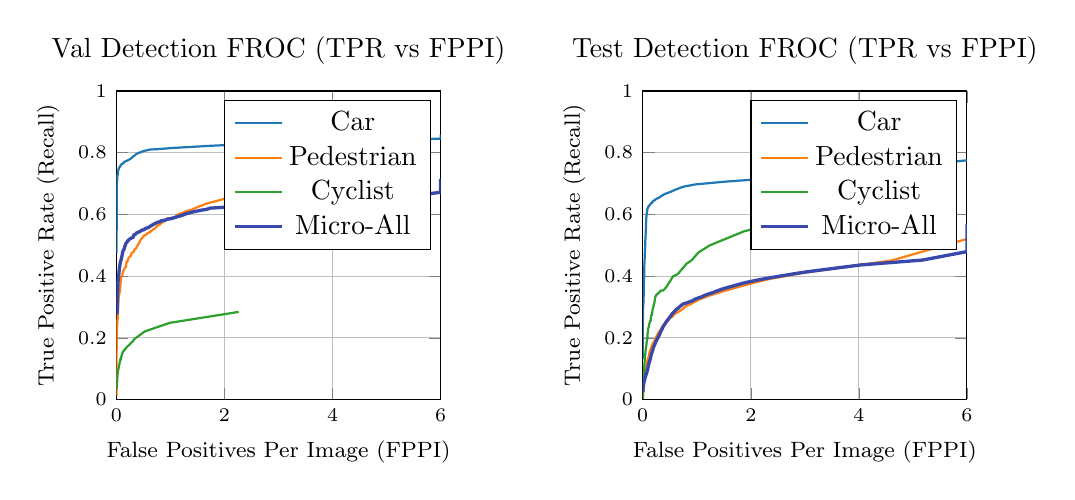
\begin{tikzpicture}
\begin{axis}[
  name=ax1, width=0.47\textwidth, height=5.5cm,
  title={Val Detection FROC (TPR vs FPPI)},
  xlabel={False Positives Per Image (FPPI)}, ylabel={True Positive Rate (Recall)},
  xmin=0, xmax=6, ymin=0, ymax=1.0, grid=both,
  legend pos=north east, tick label style={font=\scriptsize}, label style={font=\footnotesize}
]
\addplot[color=cblue, thick] coordinates {(0.0028,0.4745) (0.0032,0.5319) (0.0034,0.5634) (0.0036,0.5977) (0.0037,0.6124) (0.0038,0.5482) (0.0039,0.6467) (0.0040,0.6675) (0.0041,0.6882) (0.0041,0.6786) (0.0049,0.6950) (0.0077,0.7010) (0.0113,0.7053) (0.0143,0.7121) (0.0151,0.7157) (0.0152,0.7193) (0.0167,0.7221) (0.0175,0.7233) (0.0198,0.7265) (0.0259,0.7309) (0.0282,0.7329) (0.0298,0.7384) (0.0321,0.7404) (0.0346,0.7432) (0.0354,0.7448) (0.0385,0.7456) (0.0417,0.7464) (0.0448,0.7472) (0.0449,0.7480) (0.0482,0.7504) (0.0490,0.7508) (0.0530,0.7520) (0.0619,0.7536) (0.0711,0.7568) (0.0770,0.7592) (0.0829,0.7604) (0.0896,0.7608) (0.0980,0.7624) (0.1083,0.7640) (0.1127,0.7644) (0.1224,0.7659) (0.1302,0.7663) (0.1383,0.7675) (0.1505,0.7711) (0.1630,0.7715) (0.1759,0.7723) (0.1892,0.7735) (0.2084,0.7751) (0.2259,0.7763) (0.2409,0.7783) (0.2602,0.7799) (0.2958,0.7855) (0.3277,0.7895) (0.3642,0.7955) (0.4208,0.7998) (0.5013,0.8050) (0.6214,0.8102) (0.7695,0.8114) (1.0198,0.8150) (1.6946,0.8218) (3.0469,0.8333) (6.0000,0.8453) (6.0000,0.8585)}; \addlegendentry{Car}
\addplot[color=corange, thick] coordinates {(0.0001,0.0124) (0.0002,0.0227) (0.0002,0.0159) (0.0003,0.0363) (0.0003,0.0299) (0.0013,0.0813) (0.0013,0.0710) (0.0013,0.0534) (0.0013,0.0435) (0.0014,0.0658) (0.0025,0.1400) (0.0025,0.1132) (0.0025,0.0917) (0.0026,0.1312) (0.0026,0.1212) (0.0026,0.1033) (0.0030,0.1523) (0.0041,0.1675) (0.0051,0.1886) (0.0051,0.1790) (0.0062,0.2105) (0.0062,0.1990) (0.0099,0.2241) (0.0130,0.2360) (0.0150,0.2440) (0.0187,0.2520) (0.0210,0.2580) (0.0219,0.2608) (0.0243,0.2679) (0.0246,0.2711) (0.0281,0.2783) (0.0308,0.2871) (0.0315,0.2963) (0.0351,0.3058) (0.0353,0.3126) (0.0384,0.3214) (0.0401,0.3274) (0.0429,0.3325) (0.0472,0.3381) (0.0551,0.3441) (0.0627,0.3501) (0.0654,0.3557) (0.0678,0.3628) (0.0713,0.3676) (0.0736,0.3732) (0.0797,0.3804) (0.0808,0.3856) (0.0851,0.3911) (0.0921,0.3963) (0.1000,0.3979) (0.1086,0.4031) (0.1124,0.4075) (0.1179,0.4111) (0.1207,0.4143) (0.1309,0.4175) (0.1412,0.4215) (0.1522,0.4254) (0.1628,0.4282) (0.1692,0.4290) (0.1749,0.4290) (0.1879,0.4474) (0.1961,0.4474) (0.2038,0.4474) (0.2104,0.4506) (0.2172,0.4553) (0.2248,0.4589) (0.2378,0.4609) (0.2473,0.4625) (0.2584,0.4649) (0.2667,0.4661) (0.2746,0.4709) (0.2794,0.4745) (0.3216,0.4789) (0.3235,0.4817) (0.3320,0.4848) (0.3446,0.4872) (0.3544,0.4884) (0.3657,0.4904) (0.3803,0.4964) (0.3905,0.4996) (0.4051,0.5028) (0.4166,0.5068) (0.4288,0.5104) (0.4376,0.5148) (0.4491,0.5171) (0.4641,0.5211) (0.4736,0.5239) (0.4952,0.5263) (0.5067,0.5315) (0.5308,0.5335) (0.5549,0.5347) (0.5686,0.5383) (0.5920,0.5407) (0.6117,0.5411) (0.6343,0.5455) (0.6648,0.5486) (0.6851,0.5518) (0.7062,0.5534) (0.7314,0.5578) (0.7609,0.5638) (0.7901,0.5654) (0.8216,0.5706) (0.8559,0.5750) (0.8824,0.5774) (0.9243,0.5817) (0.9320,0.5865) (1.0915,0.5901) (1.0989,0.5941) (1.1363,0.5997) (1.2107,0.6041) (1.2983,0.6108) (1.3973,0.6156) (1.5139,0.6248) (1.6730,0.6352) (1.8813,0.6447) (2.1920,0.6603) (2.8545,0.6766) (5.7788,0.7301) (5.7788,0.7301)}; \addlegendentry{Pedestrian}
\addplot[color=cgreen, thick] coordinates {(0.0001,0.0435) (0.0001,0.0359) (0.0001,0.0303) (0.0066,0.0467) (0.0099,0.0546) (0.0135,0.0586) (0.0148,0.0650) (0.0149,0.0598) (0.0172,0.0710) (0.0184,0.0781) (0.0184,0.0738) (0.0223,0.0849) (0.0249,0.0873) (0.0272,0.0877) (0.0294,0.0889) (0.0302,0.0889) (0.0305,0.0897) (0.0318,0.0973) (0.0348,0.0981) (0.0382,0.0997) (0.0399,0.1009) (0.0426,0.1041) (0.0427,0.1053) (0.0436,0.1061) (0.0461,0.1089) (0.0462,0.1112) (0.0463,0.1085) (0.0468,0.1128) (0.0488,0.1128) (0.0505,0.1128) (0.0523,0.1136) (0.0567,0.1152) (0.0602,0.1192) (0.0631,0.1208) (0.0632,0.1220) (0.0657,0.1260) (0.0690,0.1264) (0.0718,0.1300) (0.0758,0.1300) (0.0792,0.1300) (0.0833,0.1352) (0.0877,0.1380) (0.0929,0.1392) (0.0968,0.1415) (0.0970,0.1431) (0.1016,0.1463) (0.1078,0.1483) (0.1134,0.1511) (0.1208,0.1539) (0.1319,0.1579) (0.1451,0.1591) (0.1569,0.1627) (0.1735,0.1655) (0.1865,0.1691) (0.2179,0.1746) (0.2417,0.1774) (0.2701,0.1842) (0.2976,0.1870) (0.3330,0.1962) (0.3934,0.2037) (0.5224,0.2205) (0.9865,0.2484) (2.2626,0.2839)}; \addlegendentry{Cyclist}
\addplot[color=call, very thick] coordinates {(0.0102,0.2763) (0.0126,0.2839) (0.0138,0.2936) (0.0144,0.3008) (0.0177,0.3090) (0.0200,0.3261) (0.0201,0.3387) (0.0201,0.3179) (0.0202,0.3341) (0.0214,0.3450) (0.0238,0.3527) (0.0250,0.3605) (0.0251,0.3664) (0.0258,0.3773) (0.0258,0.3714) (0.0297,0.3814) (0.0330,0.3885) (0.0375,0.3957) (0.0414,0.4011) (0.0441,0.4061) (0.0478,0.4119) (0.0494,0.4171) (0.0545,0.4234) (0.0579,0.4289) (0.0604,0.4327) (0.0644,0.4365) (0.0682,0.4401) (0.0704,0.4417) (0.0735,0.4451) (0.0757,0.4472) (0.0827,0.4507) (0.0914,0.4551) (0.0956,0.4599) (0.1008,0.4642) (0.1034,0.4673) (0.1094,0.4714) (0.1125,0.4757) (0.1162,0.4786) (0.1219,0.4810) (0.1324,0.4848) (0.1409,0.4876) (0.1463,0.4903) (0.1496,0.4935) (0.1546,0.4955) (0.1582,0.4977) (0.1653,0.5008) (0.1686,0.5032) (0.1754,0.5059) (0.1837,0.5080) (0.1924,0.5089) (0.2023,0.5113) (0.2081,0.5136) (0.2166,0.5151) (0.2200,0.5164) (0.2322,0.5179) (0.2447,0.5199) (0.2620,0.5218) (0.2803,0.5235) (0.2913,0.5245) (0.3057,0.5252) (0.3221,0.5333) (0.3328,0.5341) (0.3440,0.5346) (0.3560,0.5363) (0.3659,0.5388) (0.3780,0.5402) (0.3965,0.5412) (0.4080,0.5426) (0.4282,0.5441) (0.4451,0.5453) (0.4588,0.5471) (0.4682,0.5487) (0.5134,0.5504) (0.5223,0.5524) (0.5377,0.5542) (0.5547,0.5555) (0.5724,0.5562) (0.5932,0.5574) (0.6116,0.5601) (0.6305,0.5620) (0.6525,0.5645) (0.6720,0.5661) (0.6887,0.5679) (0.7085,0.5702) (0.7267,0.5714) (0.7467,0.5732) (0.7706,0.5749) (0.8097,0.5762) (0.8284,0.5790) (0.8612,0.5804) (0.9016,0.5812) (0.9246,0.5831) (0.9648,0.5851) (1.0004,0.5856) (1.0396,0.5878) (1.0980,0.5905) (1.1378,0.5934) (1.1819,0.5950) (1.2326,0.5980) (1.2875,0.6020) (1.3408,0.6042) (1.4079,0.6076) (1.4946,0.6107) (1.5645,0.6135) (1.6673,0.6161) (1.7366,0.6202) (1.9830,0.6228) (2.0725,0.6245) (2.2035,0.6275) (2.4099,0.6314) (2.6511,0.6349) (3.0245,0.6387) (3.6019,0.6446) (4.4586,0.6519) (5.4506,0.6602) (6.0000,0.6713) (6.0000,0.6825) (6.0000,0.7149) (6.0000,0.7149)}; \addlegendentry{Micro-All}
\end{axis}

\begin{axis}[
  at={($(ax1.outer south east)+(0.5cm,0)$)}, anchor=outer south west,
  width=0.47\textwidth, height=5.5cm,
  title={Test Detection FROC (TPR vs FPPI)},
  xlabel={False Positives Per Image (FPPI)}, ylabel={True Positive Rate (Recall)},
  xmin=0, xmax=6, ymin=0, ymax=1.0, grid=both,
  legend pos=north east, tick label style={font=\scriptsize}, label style={font=\footnotesize}
]
\addplot[color=cblue, thick] coordinates {(0.0004,0.1328) (0.0007,0.2141) (0.0008,0.2396) (0.0032,0.2723) (0.0043,0.2847) (0.0070,0.2939) (0.0078,0.3018) (0.0114,0.3102) (0.0129,0.3142) (0.0161,0.3289) (0.0177,0.3549) (0.0202,0.3716) (0.0233,0.3900) (0.0276,0.4011) (0.0282,0.4258) (0.0283,0.4115) (0.0284,0.4314) (0.0319,0.4438) (0.0323,0.4486) (0.0347,0.4561) (0.0364,0.4597) (0.0383,0.4713) (0.0407,0.4769) (0.0426,0.4841) (0.0457,0.5068) (0.0490,0.5195) (0.0539,0.5383) (0.0589,0.5586) (0.0617,0.5738) (0.0648,0.5845) (0.0676,0.5921) (0.0709,0.5977) (0.0736,0.6041) (0.0780,0.6069) (0.0814,0.6116) (0.0839,0.6148) (0.0884,0.6176) (0.0916,0.6200) (0.0989,0.6224) (0.1018,0.6248) (0.1087,0.6256) (0.1166,0.6276) (0.1247,0.6296) (0.1325,0.6308) (0.1381,0.6324) (0.1459,0.6340) (0.1578,0.6368) (0.1679,0.6372) (0.1785,0.6404) (0.1896,0.6427) (0.2038,0.6447) (0.2217,0.6459) (0.2486,0.6499) (0.2784,0.6527) (0.2995,0.6539) (0.3420,0.6591) (0.3841,0.6639) (0.4304,0.6675) (0.5056,0.6722) (0.6005,0.6798) (0.7465,0.6894) (0.9686,0.6970) (1.5021,0.7057) (3.0084,0.7249) (6.0000,0.7751) (6.0000,0.7751)}; \addlegendentry{Car}
\addplot[color=corange, thick] coordinates {(0.0002,0.0028) (0.0002,0.0028) (0.0004,0.0048) (0.0012,0.0080) (0.0015,0.0112) (0.0035,0.0144) (0.0040,0.0243) (0.0041,0.0195) (0.0052,0.0263) (0.0072,0.0323) (0.0091,0.0375) (0.0136,0.0435) (0.0155,0.0514) (0.0199,0.0582) (0.0254,0.0662) (0.0332,0.0746) (0.0363,0.0829) (0.0510,0.0925) (0.0595,0.1009) (0.0681,0.1108) (0.0779,0.1208) (0.0932,0.1304) (0.1069,0.1368) (0.1145,0.1443) (0.1246,0.1515) (0.1351,0.1591) (0.1553,0.1675) (0.1681,0.1738) (0.1807,0.1794) (0.2002,0.1854) (0.2190,0.1902) (0.2334,0.1962) (0.2473,0.2022) (0.2633,0.2073) (0.2789,0.2133) (0.2998,0.2189) (0.3234,0.2253) (0.3457,0.2305) (0.3649,0.2376) (0.3857,0.2424) (0.4036,0.2456) (0.4303,0.2488) (0.4562,0.2524) (0.4783,0.2584) (0.5045,0.2640) (0.5374,0.2675) (0.5721,0.2735) (0.6065,0.2791) (0.6500,0.2831) (0.6933,0.2879) (0.7348,0.2927) (0.7733,0.2990) (0.8264,0.3046) (0.8921,0.3094) (0.9535,0.3158) (1.0356,0.3234) (1.1114,0.3285) (1.2244,0.3361) (1.3441,0.3429) (1.5081,0.3517) (1.7008,0.3612) (1.9560,0.3736) (2.3040,0.3892) (2.9356,0.4091) (4.6067,0.4506) (6.0000,0.5203)}; \addlegendentry{Pedestrian}
\addplot[color=cgreen, thick] coordinates {(0.0001,0.0028) (0.0018,0.0048) (0.0024,0.0072) (0.0038,0.0152) (0.0097,0.0295) (0.0140,0.0470) (0.0185,0.0650) (0.0230,0.0845) (0.0282,0.1057) (0.0332,0.1212) (0.0407,0.1376) (0.0500,0.1523) (0.0589,0.1679) (0.0643,0.1738) (0.0684,0.1786) (0.0712,0.1842) (0.0802,0.1918) (0.0861,0.1998) (0.0884,0.2105) (0.0944,0.2201) (0.1008,0.2265) (0.1062,0.2337) (0.1149,0.2372) (0.1209,0.2456) (0.1285,0.2496) (0.1369,0.2536) (0.1464,0.2556) (0.1519,0.2687) (0.1597,0.2739) (0.1693,0.2751) (0.1758,0.2787) (0.1791,0.2887) (0.1845,0.2935) (0.1898,0.2967) (0.1968,0.3006) (0.2020,0.3046) (0.2094,0.3102) (0.2170,0.3146) (0.2213,0.3214) (0.2337,0.3329) (0.2434,0.3361) (0.2530,0.3397) (0.2686,0.3413) (0.2913,0.3449) (0.3115,0.3485) (0.3380,0.3533) (0.3578,0.3533) (0.3749,0.3533) (0.3968,0.3565) (0.4177,0.3608) (0.4357,0.3644) (0.4578,0.3700) (0.4744,0.3760) (0.4983,0.3812) (0.5200,0.3876) (0.5408,0.3935) (0.5581,0.3987) (0.5867,0.4015) (0.6202,0.4043) (0.6556,0.4075) (0.7038,0.4187) (0.7567,0.4282) (0.8094,0.4402) (0.9041,0.4510) (1.0308,0.4765) (1.2447,0.5000) (1.8814,0.5455) (3.7961,0.6268)}; \addlegendentry{Cyclist}
\addplot[color=call, very thick] coordinates {(0.0037,0.0237) (0.0066,0.0374) (0.0128,0.0466) (0.0208,0.0536) (0.0269,0.0593) (0.0360,0.0648) (0.0441,0.0703) (0.0532,0.0756) (0.0648,0.0823) (0.0776,0.0895) (0.0908,0.0980) (0.1010,0.1070) (0.1116,0.1157) (0.1255,0.1239) (0.1436,0.1325) (0.1492,0.1407) (0.1639,0.1501) (0.1849,0.1594) (0.1943,0.1681) (0.2186,0.1765) (0.2397,0.1862) (0.2624,0.1942) (0.2844,0.2010) (0.3034,0.2081) (0.3238,0.2162) (0.3536,0.2268) (0.3764,0.2358) (0.4058,0.2435) (0.4295,0.2504) (0.4568,0.2571) (0.4820,0.2622) (0.5055,0.2680) (0.5284,0.2738) (0.5531,0.2792) (0.5847,0.2847) (0.6112,0.2905) (0.6501,0.2954) (0.6840,0.3009) (0.7197,0.3060) (0.7560,0.3100) (0.8036,0.3124) (0.8581,0.3161) (0.9240,0.3202) (0.9685,0.3252) (1.0277,0.3291) (1.0914,0.3327) (1.1534,0.3381) (1.2213,0.3424) (1.2927,0.3461) (1.3636,0.3511) (1.4439,0.3563) (1.5257,0.3608) (1.6393,0.3662) (1.7494,0.3717) (1.8647,0.3774) (2.0113,0.3830) (2.1856,0.3892) (2.3896,0.3955) (2.6600,0.4034) (2.9787,0.4124) (3.4137,0.4223) (4.0403,0.4362) (5.1790,0.4519) (6.0000,0.4793) (6.0000,0.5674) (6.0000,0.5674)}; \addlegendentry{Micro-All}
\end{axis}
\end{tikzpicture}
\end{center}

\begin{center}
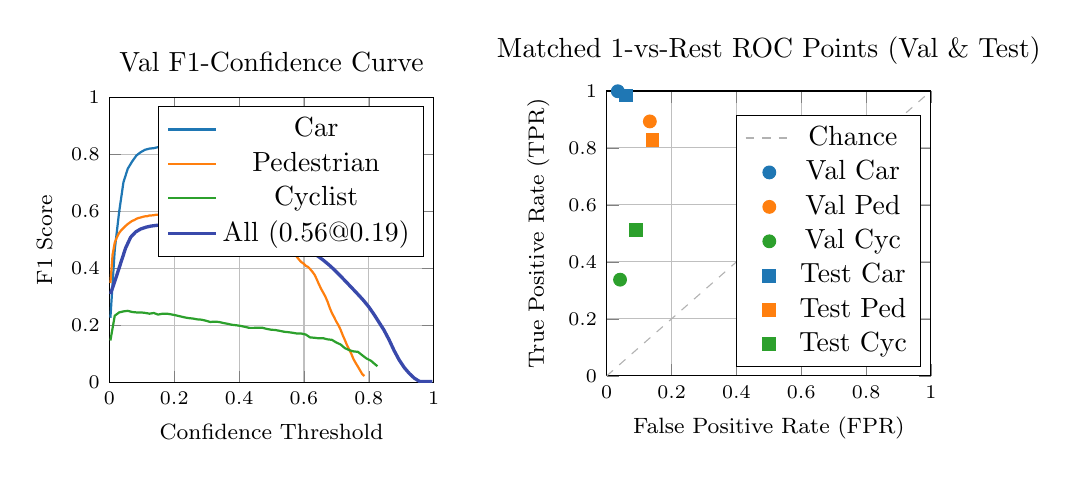
\begin{tikzpicture}
\begin{axis}[
  name=ax3, width=0.47\textwidth, height=5.2cm,
  title={Val F1-Confidence Curve},
  xlabel={Confidence Threshold}, ylabel={F1 Score},
  xmin=0, xmax=1, ymin=0, ymax=1.0, grid=both,
  legend pos=north east, tick label style={font=\scriptsize}, label style={font=\footnotesize}
]
\addplot[color=cblue, thick] coordinates {(0.0030,0.2277) (0.0164,0.4665) (0.0298,0.5981) (0.0432,0.7033) (0.0565,0.7508) (0.0699,0.7759) (0.0833,0.7974) (0.0967,0.8090) (0.1101,0.8174) (0.1235,0.8214) (0.1369,0.8230) (0.1503,0.8266) (0.1637,0.8289) (0.1771,0.8305) (0.1905,0.8333) (0.2039,0.8341) (0.2173,0.8377) (0.2307,0.8389) (0.2440,0.8405) (0.2574,0.8417) (0.2708,0.8425) (0.2842,0.8437) (0.2976,0.8441) (0.3110,0.8449) (0.3244,0.8457) (0.3378,0.8469) (0.3512,0.8473) (0.3646,0.8477) (0.3780,0.8481) (0.3914,0.8473) (0.4048,0.8473) (0.4182,0.8481) (0.4315,0.8481) (0.4449,0.8481) (0.4583,0.8469) (0.4717,0.8465) (0.4851,0.8469) (0.4985,0.8469) (0.5119,0.8469) (0.5253,0.8461) (0.5387,0.8445) (0.5521,0.8409) (0.5655,0.8401) (0.5789,0.8385) (0.5923,0.8369) (0.6057,0.8353) (0.6190,0.8345) (0.6324,0.8325) (0.6458,0.8301) (0.6592,0.8266) (0.6726,0.8246) (0.6860,0.8198) (0.6994,0.8170) (0.7128,0.8122) (0.7262,0.8034) (0.7396,0.7963) (0.7530,0.7851) (0.7664,0.7648) (0.7798,0.7472) (0.7932,0.7289) (0.8065,0.7073) (0.8199,0.6754) (0.8266,0.6423)}; \addlegendentry{Car}
\addplot[color=corange, thick] coordinates {(0.0030,0.3497) (0.0097,0.4490) (0.0164,0.4916) (0.0231,0.5104) (0.0298,0.5251) (0.0365,0.5351) (0.0432,0.5427) (0.0499,0.5502) (0.0565,0.5566) (0.0632,0.5622) (0.0699,0.5674) (0.0766,0.5706) (0.0833,0.5750) (0.0900,0.5781) (0.0967,0.5797) (0.1034,0.5821) (0.1101,0.5837) (0.1168,0.5841) (0.1235,0.5869) (0.1302,0.5869) (0.1369,0.5877) (0.1436,0.5893) (0.1503,0.5897) (0.1570,0.5921) (0.1637,0.5925) (0.1704,0.5945) (0.1771,0.5965) (0.1838,0.5957) (0.1905,0.5989) (0.1972,0.6005) (0.2039,0.5989) (0.2106,0.6001) (0.2173,0.5993) (0.2240,0.5985) (0.2307,0.5989) (0.2374,0.5965) (0.2440,0.5957) (0.2507,0.5941) (0.2574,0.5937) (0.2641,0.5933) (0.2708,0.5905) (0.2775,0.5905) (0.2842,0.5909) (0.2909,0.5909) (0.2976,0.5913) (0.3043,0.5909) (0.3110,0.5885) (0.3177,0.5885) (0.3244,0.5853) (0.3311,0.5857) (0.3378,0.5861) (0.3445,0.5861) (0.3512,0.5865) (0.3579,0.5845) (0.3646,0.5813) (0.3713,0.5789) (0.3780,0.5770) (0.3847,0.5758) (0.3914,0.5746) (0.3981,0.5726) (0.4048,0.5698) (0.4115,0.5682) (0.4182,0.5662) (0.4249,0.5646) (0.4315,0.5630) (0.4382,0.5606) (0.4449,0.5582) (0.4516,0.5546) (0.4583,0.5506) (0.4650,0.5506) (0.4717,0.5463) (0.4784,0.5415) (0.4851,0.5363) (0.4918,0.5299) (0.4985,0.5243) (0.5052,0.5215) (0.5119,0.5207) (0.5186,0.5064) (0.5253,0.5020) (0.5320,0.4968) (0.5387,0.4912) (0.5454,0.4856) (0.5521,0.4793) (0.5588,0.4701) (0.5655,0.4617) (0.5722,0.4514) (0.5789,0.4402) (0.5856,0.4306) (0.5923,0.4226) (0.5990,0.4179) (0.6057,0.4099) (0.6124,0.4063) (0.6190,0.3987) (0.6257,0.3896) (0.6324,0.3792) (0.6391,0.3636) (0.6458,0.3461) (0.6525,0.3301) (0.6592,0.3162) (0.6659,0.3022) (0.6726,0.2847) (0.6793,0.2632) (0.6860,0.2448) (0.6927,0.2305) (0.6994,0.2149) (0.7061,0.2022) (0.7128,0.1862) (0.7195,0.1667) (0.7262,0.1495) (0.7329,0.1312) (0.7396,0.1164) (0.7463,0.1005) (0.7530,0.0821) (0.7597,0.0686) (0.7664,0.0562) (0.7731,0.0431) (0.7798,0.0299) (0.7865,0.0231) (0.7865,0.0231)}; \addlegendentry{Pedestrian}
\addplot[color=cgreen, thick] coordinates {(0.0030,0.1479) (0.0164,0.2348) (0.0298,0.2464) (0.0432,0.2500) (0.0565,0.2520) (0.0699,0.2480) (0.0833,0.2464) (0.0967,0.2464) (0.1101,0.2448) (0.1235,0.2420) (0.1369,0.2444) (0.1503,0.2388) (0.1637,0.2420) (0.1771,0.2420) (0.1905,0.2396) (0.2039,0.2364) (0.2173,0.2329) (0.2307,0.2293) (0.2440,0.2265) (0.2574,0.2249) (0.2708,0.2221) (0.2842,0.2209) (0.2976,0.2173) (0.3110,0.2129) (0.3244,0.2141) (0.3378,0.2129) (0.3512,0.2093) (0.3646,0.2065) (0.3780,0.2030) (0.3914,0.2014) (0.4048,0.1990) (0.4182,0.1958) (0.4315,0.1922) (0.4449,0.1922) (0.4583,0.1926) (0.4717,0.1926) (0.4851,0.1886) (0.4985,0.1858) (0.5119,0.1846) (0.5253,0.1818) (0.5387,0.1786) (0.5521,0.1770) (0.5655,0.1750) (0.5789,0.1722) (0.5923,0.1722) (0.6057,0.1687) (0.6190,0.1587) (0.6324,0.1575) (0.6458,0.1555) (0.6592,0.1559) (0.6726,0.1519) (0.6860,0.1503) (0.6994,0.1411) (0.7128,0.1340) (0.7262,0.1212) (0.7396,0.1140) (0.7530,0.1096) (0.7664,0.1081) (0.7798,0.0961) (0.7932,0.0845) (0.8065,0.0770) (0.8199,0.0638) (0.8266,0.0578)}; \addlegendentry{Cyclist}
\addplot[color=call, very thick] coordinates {(0.0030,0.3106) (0.0186,0.3628) (0.0342,0.4175) (0.0499,0.4725) (0.0655,0.5104) (0.0811,0.5291) (0.0967,0.5395) (0.1124,0.5455) (0.1280,0.5494) (0.1436,0.5518) (0.1592,0.5534) (0.1749,0.5546) (0.1905,0.5554) (0.2061,0.5554) (0.2217,0.5554) (0.2374,0.5546) (0.2530,0.5538) (0.2686,0.5526) (0.2842,0.5514) (0.2999,0.5506) (0.3155,0.5494) (0.3311,0.5482) (0.3467,0.5467) (0.3624,0.5447) (0.3780,0.5427) (0.3936,0.5407) (0.4092,0.5383) (0.4249,0.5355) (0.4405,0.5327) (0.4561,0.5295) (0.4717,0.5259) (0.4874,0.5219) (0.5030,0.5171) (0.5186,0.5116) (0.5342,0.5052) (0.5499,0.4980) (0.5655,0.4908) (0.5811,0.4837) (0.5967,0.4753) (0.6124,0.4657) (0.6280,0.4553) (0.6436,0.4434) (0.6592,0.4302) (0.6749,0.4155) (0.6905,0.3995) (0.7061,0.3820) (0.7217,0.3636) (0.7374,0.3449) (0.7530,0.3262) (0.7686,0.3074) (0.7842,0.2879) (0.7999,0.2659) (0.8155,0.2404) (0.8311,0.2125) (0.8467,0.1846) (0.8624,0.1507) (0.8780,0.1128) (0.8936,0.0797) (0.9092,0.0530) (0.9249,0.0323) (0.9405,0.0156) (0.9561,0.0044) (0.9717,0.0036) (0.9874,0.0036) (0.9963,0.0036)}; \addlegendentry{All (0.56@0.19)}
\end{axis}

\begin{axis}[
  at={($(ax3.outer south east)+(0.5cm,0)$)}, anchor=outer south west,
  width=0.47\textwidth, height=5.2cm,
  title={Matched 1-vs-Rest ROC Points (Val \& Test)},
  xlabel={False Positive Rate (FPR)}, ylabel={True Positive Rate (TPR)},
  xmin=0, xmax=1, ymin=0, ymax=1.0, grid=both,
  legend pos=south east, tick label style={font=\scriptsize}, label style={font=\footnotesize}
]
\addplot[color=gray!60, dashed] coordinates {(0,0) (1,1)}; \addlegendentry{Chance}
\addplot[color=cblue, only marks, mark=*, mark size=2.3pt] coordinates {(0.0341,0.9989)}; \addlegendentry{Val Car}
\addplot[color=corange, only marks, mark=*, mark size=2.3pt] coordinates {(0.133,0.8931)}; \addlegendentry{Val Ped}
\addplot[color=cgreen, only marks, mark=*, mark size=2.3pt] coordinates {(0.0411,0.3376)}; \addlegendentry{Val Cyc}
\addplot[color=cblue, only marks, mark=square*, mark size=2.3pt] coordinates {(0.0587,0.9842)}; \addlegendentry{Test Car}
\addplot[color=corange, only marks, mark=square*, mark size=2.3pt] coordinates {(0.1411,0.8267)}; \addlegendentry{Test Ped}
\addplot[color=cgreen, only marks, mark=square*, mark size=2.3pt] coordinates {(0.0912,0.5116)}; \addlegendentry{Test Cyc}
\end{axis}
\end{tikzpicture}
\end{center}

\section*{3. 클래스별 F1 · FROC AUC · 1-vs-Rest ROC 정량 지표 표}
\begin{center}
\small
\begin{tabular}{llrrrrrrr}
\toprule
\textbf{Split} & \textbf{Class} & \textbf{GT} & \textbf{AP@0.5} & \textbf{Peak F1 (@Conf)} & \textbf{FROC AUC (5 FPPI)} & \textbf{TPR@1/2 FPPI} & \textbf{OvR TPR} & \textbf{OvR FPR} \\
\midrule
Val  & Car        & 2,075 & 0.8235 & 0.848 (@0.37) & 0.8238 & 0.813 / 0.822 & 0.9989 & 0.0341 \\
Val  & Pedestrian & 1,777 & 0.5871 & 0.601 (@0.20) & 0.6402 & 0.587 / 0.645 & 0.8931 & 0.1330 \\
Val  & Cyclist    & 754   & 0.1598 & 0.252 (@0.06) & 0.2633 & 0.248 / 0.248 & 0.3376 & 0.0411 \\
Val  & \textbf{All / Micro} & 4,606 & \textbf{0.5235} & Macro 0.555 (@0.191) & 0.6141 & 0.585 / 0.623 & \multicolumn{2}{r}{Eval F1 = \textbf{0.5766}} \\
\midrule
Test & Car        & 1,818 & 0.6662 & 0.729 (@0.36) & 0.7094 & 0.697 / 0.716 & 0.9842 & 0.0587 \\
Test & Pedestrian & 9,044 & 0.3631 & 0.435 (@0.06) & 0.3744 & 0.320 / 0.374 & 0.8267 & 0.1411 \\
Test & Cyclist    & 817   & 0.2513 & 0.372 (@0.37) & 0.5380 & 0.461 / 0.545 & 0.5116 & 0.0912 \\
Test & \textbf{All / Micro} & 11,679 & \textbf{0.4269} & Macro 0.487 (@0.322) & 0.3728 & 0.328 / 0.381 & \multicolumn{2}{r}{Eval F1 = \textbf{0.5047}} \\
\bottomrule
\end{tabular}
\end{center}

\end{document}
